
\chapter{Analyse}


\section{Die Berechnungsdauer von MPCT ohne SDT}
Das Teil-Protokoll MPCT, das die Größe der Schnittmenge der Eingabemengen sicher berechnet, war bei den meisten meiner Tests schneller als das SDT Protokoll, wenn man die Berechnungszeiten der beiden Protokolle getrennt betrachtet.\\
\begin{figure}[H]
\begin{center}
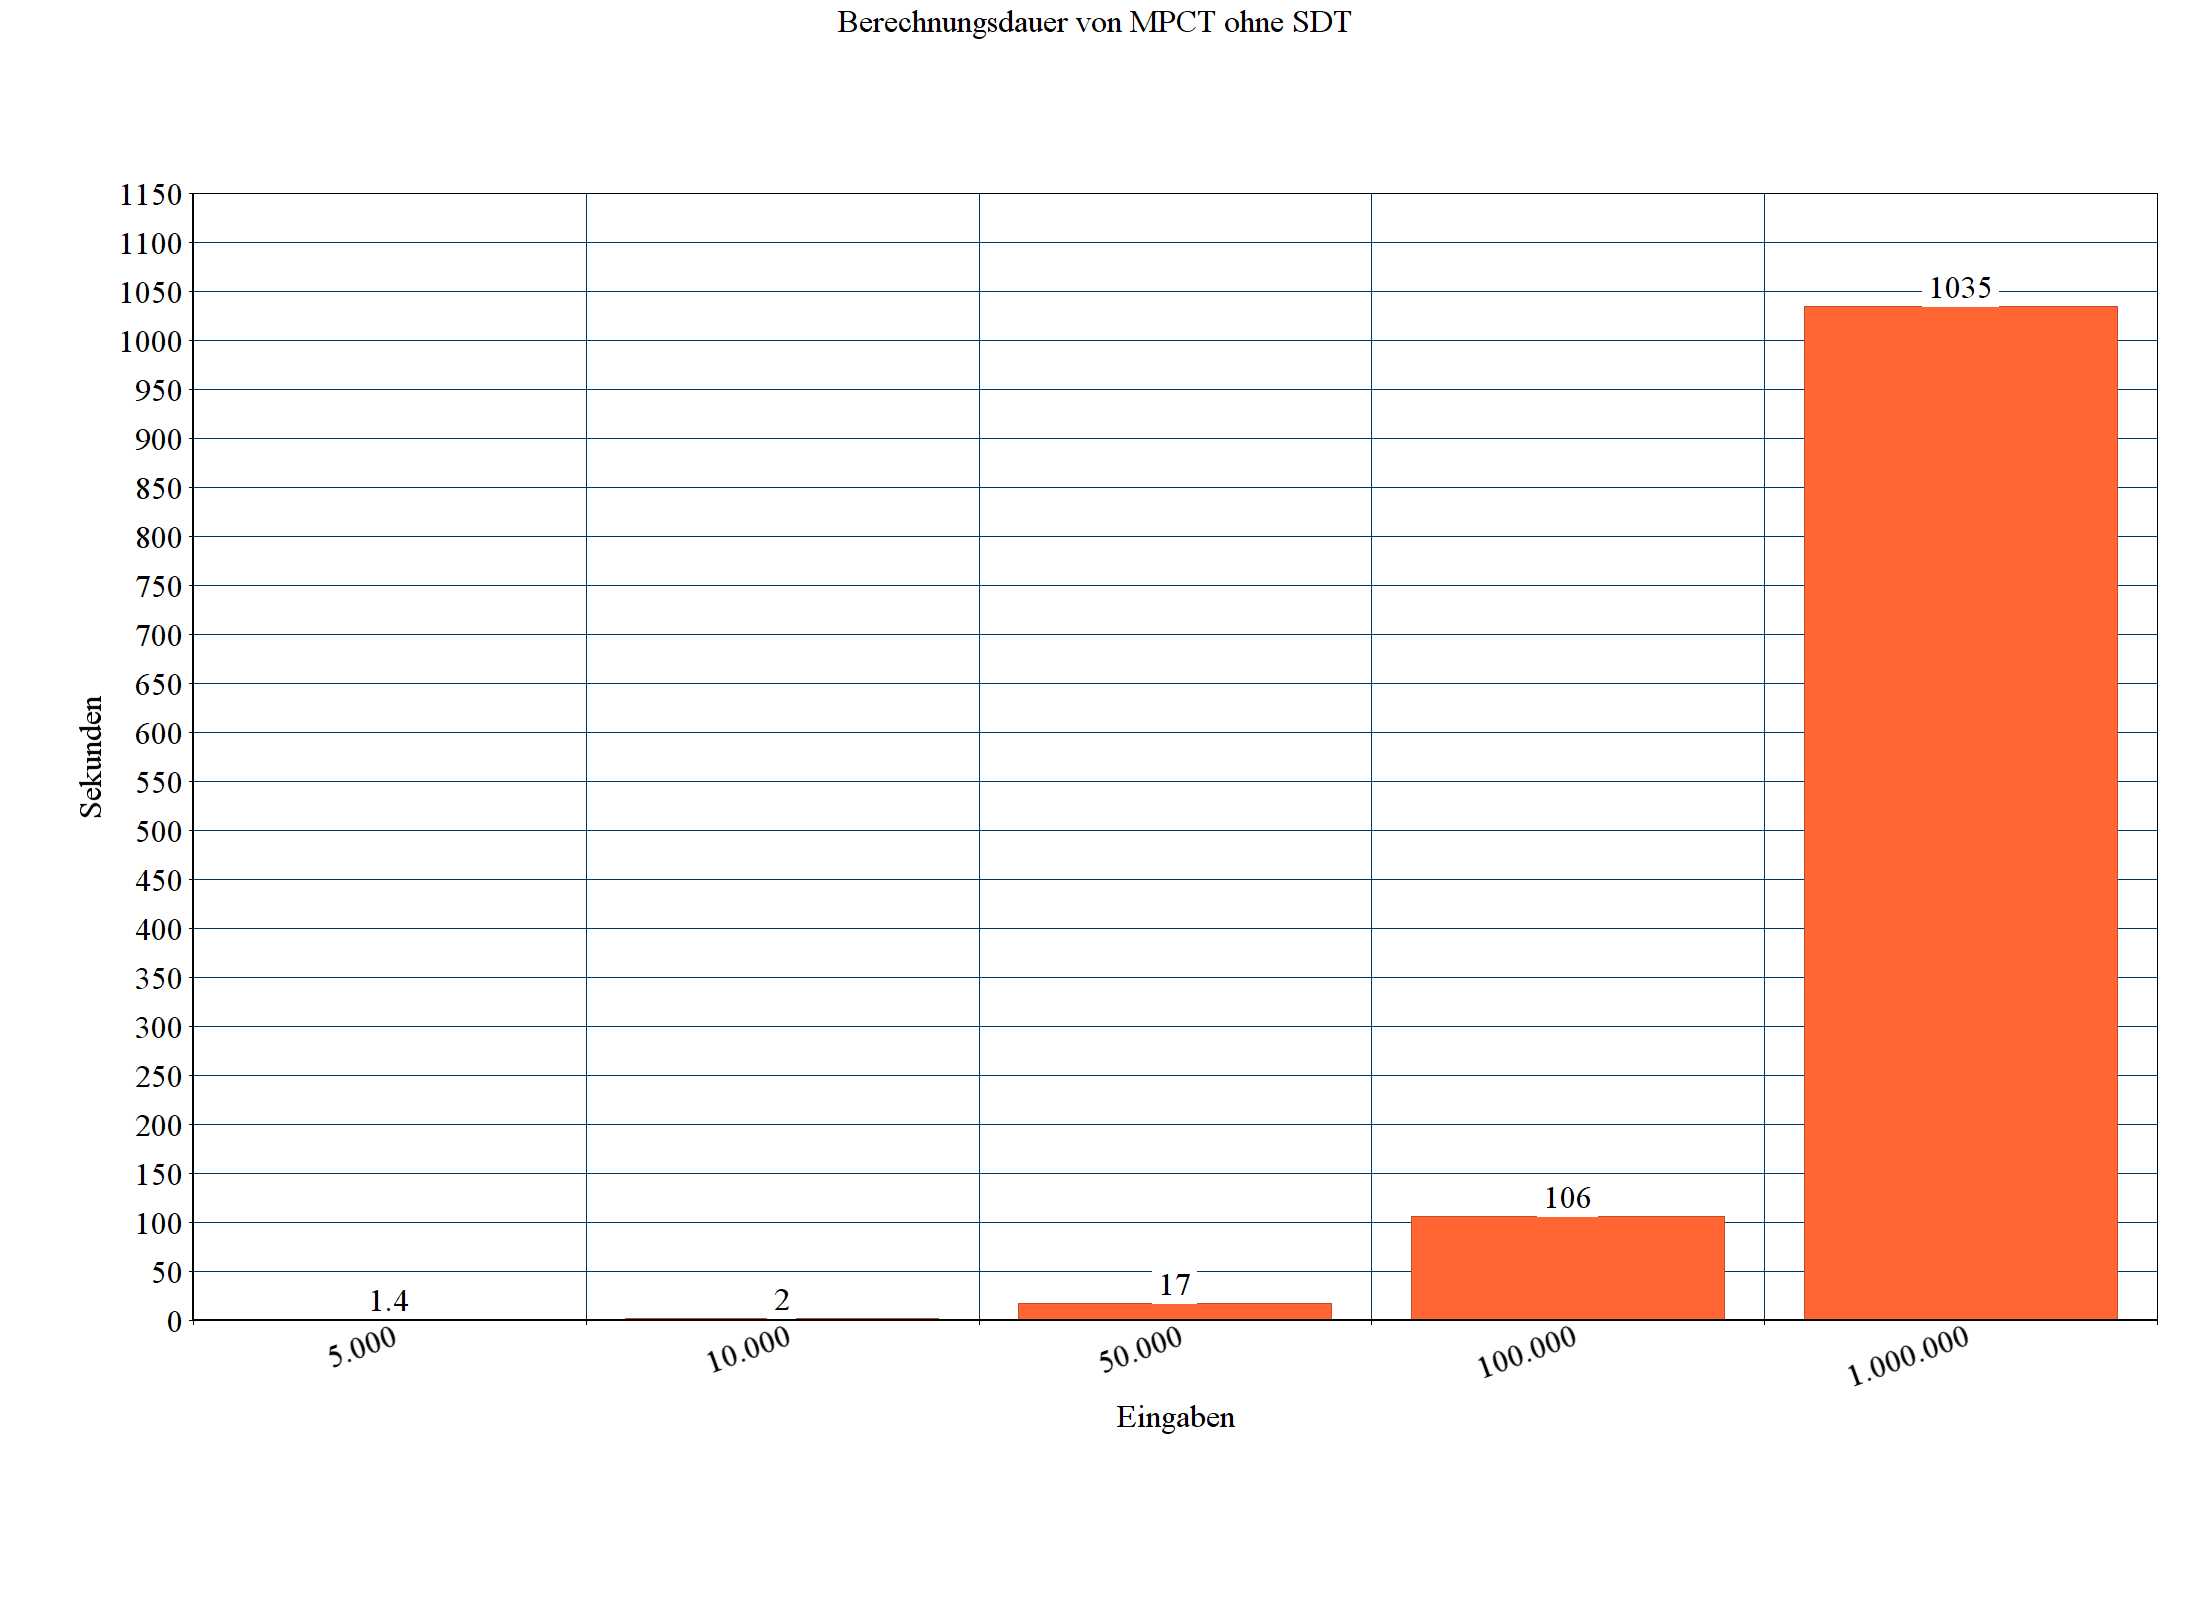
\includegraphics[width = 12cm]{MPCTTable.png}
\caption{Die Entwicklung der Berechnungsdauer von MPCT ohne SDT bei unterschiedlich vielen Eingaben}
\label{MPCTGraphic}
\end{center}

\end{figure}
In der Abbildung \ref{MPCTGraphic} ist zu erkennen, dass die Berechnungsdauer bis zu einer Eingabemenge von 100 * 100, also 10.000 Eingaben, zu vernachlässigen ist. Es ist aber auch deutlich zu sehen, dass die Berechnungsdauer von MPCT ohne SDT danach anfängt deutlich zu steigen. Bei 1.000 * 100, also einhunderttausend Eingaben ist die Berechnungsdauer stärker gestiegen als bis zu diesem Datenpunkt zu erwarten. Wenn man alle Daten betrachtet scheint der Anstieg der Berechnungsdauer zwischen linear und quadratisch zu sein.

\section{Die Berechnungsdauer von SDT}
Das Teil-Protokoll SDT, das berechnet, ob der Grad der Eingabepolynome kleiner als ein gegebener Wert ist, hat in vielen meiner Tests nur einen kleinen Teil seiner Berechnungsdauer selbst Berechnungen angestellt. Den größten Teil der Berechnungsdauer haben andere Unterprotokolle gebraucht. Diese anderen Teilprotokolle, wie OLS und secRank, sind sehr rechenintensiv. Vor allem, da sie nicht wie im Paper beschrieben implementiert werden konnten. Wenn man aber die Berechnungszeit der anderen Teilprotokolle abzieht, kann man einen besseren Überblick erhalten, wie effizient SDT ist.

\begin{figure}[H]
\begin{center}
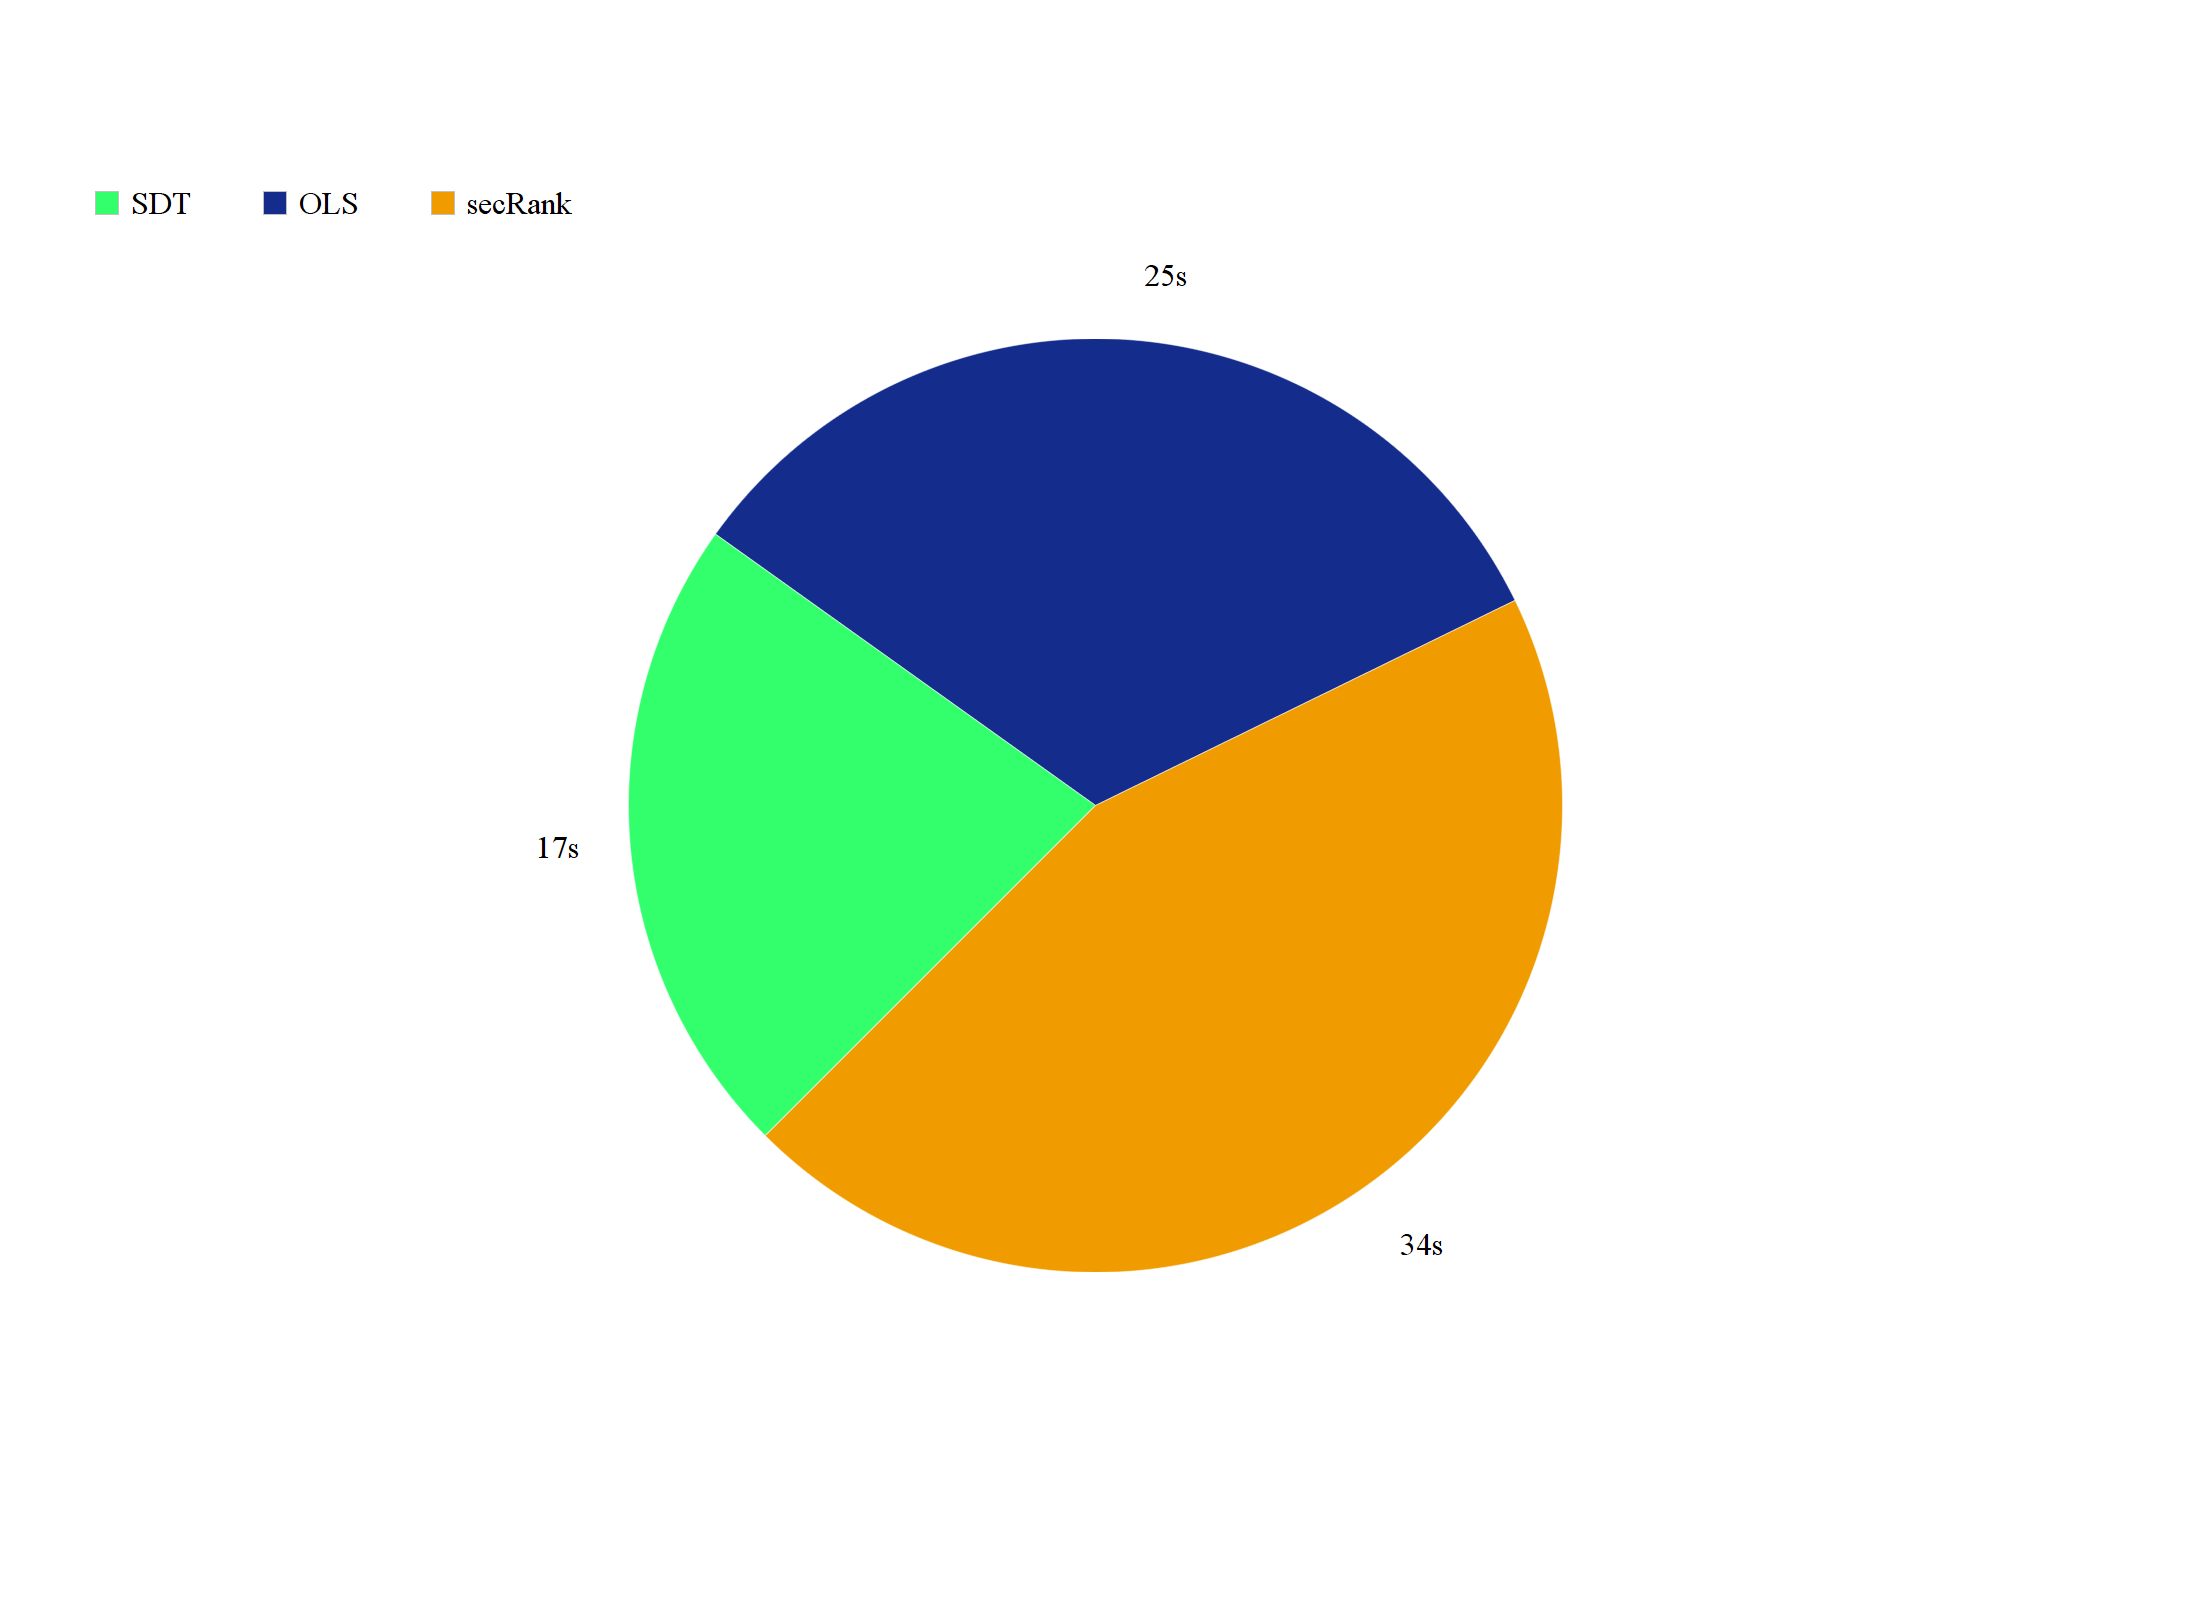
\includegraphics[width = 12cm]{SDTGraphic.png}
\caption{Die Aufteilung der Berechnungszeit von SDT im Test Big. Die Gesamtdauer von SDT beträgt 76 Sekunden}
\label{SDTGraphic}
\end{center}
\end{figure}

76 Sekunden hat die die Berechnung von SDT bei dem Test Big insgesamt gedauert. Die Berechnung der vier Aufrufe von secRank hat rund 34 Sekunden gedauert und die Berechnung der zwei Aufrufe von OLS rund 25 Sekunden. Wenn man also die Berechnungszeit der beiden ineffizient implementierten Teilprotokolle abzieht, benötigt SDT nur rund 17 Sekunden um das Ergebnis der 42 verschlüsselten Eingaben zu berechnen. Diese 42 verschlüsselten Eingaben entsprechen ebenfalls den fast 10.000 Eingaben, die MPCT erhalten hat. In der Graphik \ref{SDTGraphic} ist gut zu erkennen, dass die internen Berechnungen von SDT nur ungefähr ein Viertel der gesamten Berechnungszeit von SDT ausmacht. Andere Tests liefern ähnliche Ergebnisse. Daher hängt die Gesamtberechnungsdauer von SDT vor allem von OLS und secRank und deren Effizienz ab.

\section{Die Berechnungen in beiden Protokollen}
Im Folgenden werden die Berechnungen in MPCT und SDT und den darin enthaltenen Aufrufen von secMult zusammen betrachtet. 
Die Berechnungen in den anderen Teilprotokollen OLS und secRank werden nicht analysiert, weil sie nicht wie im Paper \cite{Doettling2021} beschrieben implementiert wurden.

   \begin{table}[!h]
     \centering
     \begin{tabular}{c|ccc|ccc}
       \textbf{Testname} & \textbf{N} & \textbf{n} & \textbf{t} & \textbf{decrypt} &\textbf{encrypt} & \textbf{Berechnungen}\\
       Basic & 2 & 5 & 2 & 8 & 86 & 378\\
       10Numbers & 2 & 10 & 2 & 8 & 86 & 378\\
       4Threshold & 2 & 5 & 4 & 8 & 126 & 618\\
       BigThreshold & 2 & 11 & 10 & 8 & 246 & 1722\\
       10Parties & 10 & 5 & 2 & 40 & 790 & 12058\\
       Big &40 & 99 & 10 & 160 & 11646 & 670826\\
     \end{tabular}

     \caption{Tabelle der Testergebnisse}
     \label{tbl:results}
     % Verweis im Text mittels \ref{tbl:beispieltabelle}

   \end{table}

\subsection{Erklärung der Ergebnistabelle}
In der Tabelle \ref{tbl:results} ist eine Übersicht über einige der angestellten Tests zu sehen. Die Tabelle ist aufgeteilt in drei Abschnitte. Die Namen der Tests, die Eingaben und die Analyseergebnisse der Tests.\\
In der Spalte \glqq N\grqq{}  ist aufgelistet, wie viele Parteien an den jeweiligen Tests teilnehmen, also wie viele ihre Eingabemengen zur Berechnung dazugeben und an der Berechnung teilnehmen.\\
Die Spalte \glqq n\grqq{} gibt die Mengengröße pro Partei an, also wie viele Zahlen in jeder der Eingabemengen sind.\\
Der \glqq threshold\grqq{} t ist etwas schwieriger zu verstehen. Die Schnittmenge der Eingaben muss größer als n(Mengengröße) - t (threshold) sein. Anders gesagt, ist der threshold so etwas, wie die Anzahl der erlaubten Abweichungen zwischen den unterschiedlichen Eingabemengen.\\
Die Spalte \glqq decrypt\grqq{} gibt die Anzahl der eher teuren Entschlüsselungen in den betrachteten Protokollen zusammen an und \glqq encrypt\grqq{} die Zahl der eher schnellen Verschlüsselungen.\\
In der Spalte Berechnungen werden alle Berechnungen mit verschlüsselten Zahlen gezählt, also die Additionen und Subtraktionen der homomorphen Verschlüsselung, sowie das Erstellen von neuen verschlüsselten Zahlen.\\
Die Anzahl der Aufrufe von OLS und secRank verändern sich bei unterschiedlichen Eingabeparametern nicht und daher sind sie nicht in der Tabelle aufgelistet.\\

\subsection{Analyse der Testergebnisse}
In der Tabelle \ref{tbl:results} kann man gut die Auswirkungen der unterschiedlichen Eingabeparameter auf die Anzahl der unterschiedlichen Berechnungen in den betrachteten Protokollen, und damit auf die Berechnungszeit der betrachteten Protokolle vergleichen.\\
Wie an Test 10Numbers zu sehen ist, hat die Größe der Eingabemengen keine Auswirkungen auf die Anzahl der Verschlüsselungen oder Entschlüsselungen in den beiden getesteten Protokollen. Auch die Anzahl der verschlüsselten Berechnungen verändert sich nicht, wenn die Eingabemengen größer werden.\\ Die Berechnungszeit im Teilprotokoll MPCT steigt jedoch trotzdem an, da dort einige Berechnungen von unverschlüsselten Daten hinzukommen. Die zeitlichen Auswirkungen die dadurch entstehen sind jedoch deutlich geringer als die Veränderungen, die durch die anderen Parameter ausgelöst werden.\\
Im Gegensatz dazu hat die Veränderung der Anzahl der beteiligten Parteien eine größere Auswirkung auf die Kosten der Protokolle. Wie zu sehen bei dem Test 10Parties hat die Vergrößerung der Anzahl der teilnehmenden Parteien auch die Anzahl an Verschlüsselungen deutlich erhöht. Die Anzahl der Verschlüsselungen und die der verschlüsselten Berechnungen steigt mit zusätzlichen Teilnehmern deutlich an. Die Steigerung ist sogar größer als die Steigerung, die bei einer Veränderung des thresholds auftritt.\\
Das ist erkennbar, wenn man die beiden Tests 10Parties und BigTreshold vergleicht. Um die erlaubten Abweichungen im Test BigTreshold auf zehn zu erhöhen, musste ich auch die Mengengröße auf elf erhöhen, da das Protokoll nur sinnvoll für die Berechnung ist, wenn die Anzahl der erlaubten Abweichungen geringer ist als die Mengengröße. Sonst wären die Eingaben der Teilnehmer irrelevant, da auch bei einer leeren Schnittmenge immer noch die Anzahl der erlaubten Abweichungen unterschritten würde, und so immer true zurück gegeben werden könnte, ohne die Eingaben zu betrachten.\\
Wie im vorigen Abschnitt zu sehen, verändert die Mengengröße jedoch nicht die Anzahl der Berechnungen. Dadurch wird das Ergebnis also nicht verfälscht.
Wenn man nun also die Anzahl der Verschlüsselungen der beiden Tests vergleicht, sieht man, dass eine Veränderung des threshold von Zwei auf Zehn einen geringeren Anstieg der Berechnungen nach sich zieht, als die Steigerung der Teilnehmeranzahl von Zwei auf Zehn.\\
Auch die Anzahl an kostenintensiven Entschlüsselungen steigt nur an, wenn sich die Anzahl der Parteien erhöht. Die Veränderung der Teilnehmeranzahl hat also die größten Auswirkungen auf die Berechnungskosten des Protokolls. Ein ähnliches Ergebnis ist auch in der Berechnungszeit der Protokolle zu beobachten.\\
Die Berechnungszeit der beiden Tests 10Parties und BigThreshold ist jedoch ähnlich, da die Unterprotokolle OLS und secRank im Test BigThreshold länger für ihre Berechnungen brauchen.\\
Die Veränderung der Größe des Körpers, über dem die Berechnungen stattfinden, hatte 
in meinen Tests wiederum keine messbaren Auswirkungen. Das ist auch erwartbar, denn die einzigen Berechnungen, bei denen der Körper relevant ist, sind Berechnungen mit BigIntegers. Und in diesen Berechnungen wird nur der Modulus verändert. Die Veränderungen sollten also kaum Auswirkungen auf die Berechnungszeit haben.\\

Die Berechnungszeit des komplett sicher implementierten Protokolls ist schwierig abzuschätzen, da wie in \ref{SDTGraphic} zu sehen, ein großer Teil der Berechnungszeit von SDT von der Effizienz der Teil-Protokolle OLS und secRank abhängt. Die Berechnungszeit könnte bei einer kompletten sicheren Implementierung dennoch ähnlich sein, wie die dieser Teil-Implementierung. Denn auch wenn die Berechnungen in OLS beispielsweise komplexer werden, sie verzichten auf viele zeitintensive Entschlüsselungen. Im Anhang unter \ref{tbl:Times} sind die Berechnungszeiten einiger Tests aufgelistet, um eine Vorstellung zu geben, wie lange diese Implementierung des MPCT Protokolls bei unterschiedlichen Eingabeparametern für die Berechnung braucht.

\section{Analyseergebnisse}
\subsection{Einordnung der Ergebnisse}
Bei den durchgeführten Tests wurden alle Berechnungen vom Tester ausgeführt. Wenn das Protokoll im Einsatz ist, werden diese Berechnungen jedoch auf die unterschiedlichen teilnehmenden Parteien aufgeteilt. Die Analyse im vorangegangenen Kapitel bezieht die Berechnungen von allen teilnehmenden Parteien (und dem Koordinator) mit ein. Betrachtet werden also die Gesamtkosten des Protokolls, jedoch nicht die Berechnungen pro teilnehmender Partei.\\
Wenn man davon ausgeht, dass die Berechnungen gleichmäßig auf alle Parteien aufgeteilt werden, haben wir bei dem Test BigThreshold 861 Berechnungen pro Partei. Bei dem Test 10Parties bekommen wir einen Wert von 1205 Berechnungen pro Partei. Die Veränderung der Teilnehmeranzahl hat also nicht nur große Auswirkungen auf die Anzahl der Gesamtberechnungen, sondern beeinflusst auch die Berechnungen pro Partei stärker als eine gleiche Veränderung des thresholds.\\
Die Berechnungen werden jedoch nicht ganz gleichmäßig auf die Parteien aufgeteilt, denn beide Teilprotokolle, vor allem das Teilprotokoll SDT, ist asymmetrisch. Der erste Schritt von SDT wird nur von einer einzelnen Partei berechnet, wie in Ausschnitt \ref{SDT asymetrie} zu sehen. 
\begin{lstlisting}[caption = Ausschnitt des Teilprotokolls SDT \cite{Doettling2021}, label = SDT asymetrie]
P1 sets [...] It homomorphically generates an encrypted linear system[...]
\end{lstlisting}
Daher muss eine Partei mehr Berechnungen als die anderen ausführen, alle anderen führen jedoch die genau gleiche Anzahl an Berechnungen aus. Dadurch liegt diese eine Partei etwas über dem oben angegebenen Durchschnittswert, und alle anderen etwas darunter.\\

\subsection{Aussage der Ergebnisse}
Die Berechnungszeit der Teilprotokolle MPCT und SDT hängt nicht mehr bedeutend von der Anzahl der Eingaben ab. Die Veränderung des thresholds und der Teilnehmeranzahl beeinflussen die Berechnungszeit jedoch deutlich. Sowohl die Anzahl der Gesamtberechnungen als auch die Berechnungen pro Partei werden von der Teilnehmeranzahl stärker beeinflusst, als vom threshold.\\
Das ist interessant, denn das vorstellende Paper \cite{Doettling2021} geht von einer Kommunikationskomplexität von O(Nt\textsuperscript{2}) aus. Sie steigt also mit dem threshold stärker an, als mit der Teilnehmeranzahl. Das ist jedoch kein Widerspruch, denn das Paper gibt mit O(Nt\textsuperscript{2}) nur die Menge der Kommunikation, nicht die der Berechnungen an.\\
Die Größe der Eingabemengen beeinflusst die Berechnungszeit von MPCT, aber nicht die Berechnungszeit von SDT.\\
